\documentclass[border = 5mm]{standalone}

% TikZ
\usepackage{tikz}

\begin{document}
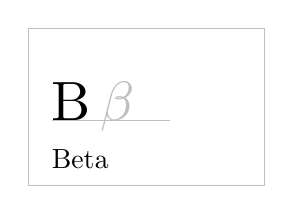
\begin{tikzpicture}
	
	\node[
		draw = gray!50,
		scale = 2,
		minimum width = 1.5cm,
		minimum height = 1cm,
		text width = 1.2cm,
		name = mynode,
	] at (0,0) {B\,$\color{gray!50}\beta$};
	
	\draw[gray!50]
		(mynode.text) to ++(1.5,0);
		
	\node[anchor = text, yshift = -6mm]
		at (mynode.text) {Beta};
	
		
\end{tikzpicture}
\end{document}